%============================================================================
% tento soubor pouzijte jako zaklad
% (c) 2008 Michal Bidlo
% E-mail: bidlom AT fit vutbr cz
%============================================================================
% kodovaní: UTF-8 (zmena prikazem iconv, recode nebo cstocs)
%----------------------------------------------------------------------------
% zpracování: make, make pdf, make desky, make clean
%============================================================================
% Šablonu upravil: Ing. Jaroslav Dytrych, idytrych@fit.vutbr.cz
%============================================================================
\documentclass[english]{fitthesis} % bez zadání - pro začátek práce, aby nebyl problém s překladem
%\documentclass[zadani]{fitthesis} % odevzdani do wisu - odkazy jsou barevné
%\documentclass[zadani,print]{fitthesis} % pro tisk - odkazy jsou černé
%\documentclass[english,print]{fitthesis} % pro tisk - odkazy jsou černé
% * Je-li prace psana v anglickem jazyce, je zapotrebi u tridy pouzit 
%   parametr english nasledovne:
%      \documentclass[english]{fitthesis}

\usepackage[czech,english]{babel}
\usepackage[utf8]{inputenc} %kodovani
\usepackage[T1]{fontenc}
\usepackage{cmap}
\usepackage{url}
\DeclareUrlCommand\url{\def\UrlLeft{<}\def\UrlRight{>} \urlstyle{tt}}

%zde muzeme vlozit vlastni balicky
\usepackage{float}
\usepackage{epstopdf}
\usepackage{amsmath,amsfonts,amssymb,amsthm}
\usepackage{listings}
\usepackage[linesnumbered, algoruled]{algorithm2e}
\usepackage[toc,page,header]{appendix}
\RequirePackage{titletoc}
\ifczech
  \usepackage{ae}
\fi

\theoremstyle{plain}
\newtheorem{thm}{Theorem}[section]
\newtheorem{lem}[thm]{Lemma}
\newtheorem{prop}[thm]{Proposition}
\newtheorem*{cor}{Corollary}

\theoremstyle{definition}
\newtheorem{defn}{Definition}[section]
\newtheorem{conj}{Conjecture}[section]
\newtheorem{exmp}{Example}[section]

\theoremstyle{remark}
\newtheorem*{rem}{Remark}
\newtheorem*{note}{Note}

%---rm---------------
\renewcommand{\rmdefault}{lmr}%zavede Latin Modern Roman jako rm
%---sf---------------
\renewcommand{\sfdefault}{qhv}%zavede TeX Gyre Heros jako sf
%---tt------------
\renewcommand{\ttdefault}{lmtt}% zavede Latin Modern tt jako tt

% vypne funkci nové šablony, která automaticky nahrazuje uvozovky,
% aby nebyly prováděny nevhodné náhrady v popisech API apod.
\csdoublequotesoff

% =======================================================================
% balíček "hyperref" vytváří klikací odkazy v pdf, pokud tedy použijeme pdflatex
% problém je, že balíček hyperref musí být uveden jako poslední, takže nemůže
% být v šabloně
\ifWis
\ifx\pdfoutput\undefined % nejedeme pod pdflatexem
\else
  \usepackage{color}
  \usepackage[unicode,colorlinks,hyperindex,plainpages=false,pdftex]{hyperref}
  \definecolor{links}{rgb}{0.4,0.5,0}
  \definecolor{anchors}{rgb}{1,0,0}
  \def\AnchorColor{anchors}
  \def\LinkColor{links}
  \def\pdfBorderAttrs{/Border [0 0 0] }  % bez okrajů kolem odkazů
  \pdfcompresslevel=9
\fi
\else % pro tisk budou odkazy, na které se dá klikat, černé
\ifx\pdfoutput\undefined % nejedeme pod pdflatexem
\else
  \usepackage{color}
  \usepackage[unicode,colorlinks,hyperindex,plainpages=false,pdftex,urlcolor=black,linkcolor=black,citecolor=black]{hyperref}
  \definecolor{links}{rgb}{0,0,0}
  \definecolor{anchors}{rgb}{0,0,0}
  \def\AnchorColor{anchors}
  \def\LinkColor{links}
  \def\pdfBorderAttrs{/Border [0 0 0] } % bez okrajů kolem odkazů
  \pdfcompresslevel=9
\fi
\fi

%Informace o praci/projektu
%---------------------------------------------------------------------------
\projectinfo{
  %Prace
  project=DP,            %typ prace BP/SP/DP/DR
  year=2016,             %rok
  date=\today,           %datum odevzdani
  %Nazev prace
  title.cs={Název práce},  %nazev prace v cestine
  title.en={Thesis title}, %nazev prace v anglictine
  %Autor
  author={Jméno Příjmení},   %jmeno prijmeni autora
  %author.title.p=Bc., %titul pred jmenem (nepovinne)
  %author.title.a=PhD, %titul za jmenem (nepovinne)
  %Ustav
  department=UITS, % doplnte prislusnou zkratku: UPSY/UIFS/UITS/UPGM
  %Skolitel
  supervisor=Jméno Příjmení, %jmeno prijmeni skolitele
  supervisor.title.p=Doc. RNDr.,   %titul pred jmenem (nepovinne)
  supervisor.title.a={Ph.D.},    %titul za jmenem (nepovinne)
  %Klicova slova, abstrakty, prohlaseni a podekovani je mozne definovat 
  %bud pomoci nasledujicich parametru nebo pomoci vyhrazenych maker (viz dale)
  %===========================================================================
  %Klicova slova
  %keywords.cs={Klíčová slova v českém jazyce.}, %klicova slova v ceskem jazyce
  %keywords.en={Klíčová slova v anglickém jazyce.}, %klicova slova v anglickem jazyce
  %Abstract
  %abstract.cs={Výtah (abstrakt) práce v českém jazyce.}, % abstrakt v ceskem jazyce
  %abstract.en={Výtah (abstrakt) práce v anglickém jazyce.}, % abstrakt v anglickem jazyce
  %Prohlaseni
  %declaration={Prohlašuji, že jsem tuto bakalářskou práci vypracoval samostatně pod vedením pana ...},
  %Podekovani (nepovinne)
  %acknowledgment={Zde je možné uvést poděkování vedoucímu práce a těm, kteří poskytli odbornou pomoc.} % nepovinne
}

%Abstrakt (cesky, anglicky)
\abstract[cs]{Do tohoto odstavce bude zapsán výtah (abstrakt) práce v českém jazyce.}
\abstract[en]{Do tohoto odstavce bude zapsán výtah (abstrakt) práce v anglickém jazyce.}

%Klicova slova (cesky, anglicky)
\keywords[cs]{Sem budou zapsána jednotlivá klíčová slova v českém jazyce, oddělená čárkami.}
\keywords[en]{Sem budou zapsána jednotlivá klíčová slova v anglickém jazyce, oddělená čárkami.}

%Prohlaseni
\declaration{Prohlašuji, že jsem tuto bakalářskou práci vypracoval samostatně pod vedením pana X...
Další informace mi poskytli...
Uvedl jsem všechny literární prameny a publikace, ze kterých jsem čerpal.}

%Podekovani (nepovinne)
\acknowledgment{V této sekci je možno uvést poděkování vedoucímu práce a těm, kteří poskytli odbornou pomoc
(externí zadavatel, konzultant, apod.).}

\begin{document}
  % Vysazeni titulnich stran
  % ----------------------------------------------
  \maketitle
  % Obsah
  % ----------------------------------------------
  \tableofcontents
  
  % Seznam obrazku a tabulek (pokud prace obsahuje velke mnozstvi obrazku, tak se to hodi)
\ifczech
  \renewcommand\listfigurename{Seznam obrázků}
\fi
  % \listoffigures
\ifczech
  \renewcommand\listtablename{Seznam tabulek}
\fi
  % \listoftables 

  % Text prace
  % ----------------------------------------------
  %=========================================================================
% (c) Michal Bidlo, Bohuslav Křena, 2008

%Cohen86 -- PhD Thesis Viruses
%Filiol12 -- Malicious cryptology and mathematics
%Moser07 -- Limits of Static Analysis for Malware Detection
%Durfina11 -- Design of a Retargetable Decompiler for a Static Platform-Independent Malware Analysis
%Konstantinou08 -- PhD Thesis Metamorphic virus
%Babic11 -- Malware detection with TA Inference
%Jacob08 -- Behavioral detection of malware: from a survey towards an established taxonomy
%You10 -- Malware Obfuscation Techniques: A Brief Survey
%Shiffman10 -- A Brief History of Malware Obfuscation
%RevGen -- Enabling sophisticated analyses of ×86 binaries with RevGen
%Christo07 -- Mining specifications of malicious behavior
%Symantec08 -- http://www.ecsl.cs.sunysb.edu/tr/TR237.pdf

\chapter{Introduction}
Information technologies and systems have found use in almost all aspects of human life. From personal communication and entertainment to industrial manufacturing, services and commerce. Because of this widespread adoption, safety and security of information systems and the data they hold has become a major concern. Throughout the years, development and administration of information systems has shown to be a complex task and errors are a common occurence. These errors may pose a safety risk to anyone using the system. Some of these errors can be abused by malicious parties to achieve goals that are not in alignment with the wishes of a legitimate user. The answer to this problem is twofold. By advancing the processes and technologies that we use to develop information systems we lower the number of errors and weaknesses that the system has prior to it's use. By carefully monitoring usage of the system after deployment, we lower the risk of abuse of errors that were not corrected during developement.

\emph{Malware} is a term used to describe any software tools primarily designed for malicious use against a host information system. Common uses include causing damage to the host system, denying usage of the host to legitimate users and theft of data and computing resources. Depending on it's purpose and method of transfer, malware can be classified into several families. For example a \emph{trojan} is malware that is introduced into a host, often by a legitimate user, disguising itself as harmless software. On the other hand a \emph{worm} often abuses an error in the host system to gain access. Both of these are examples of malware that function as standalone pieces of software. \emph{Viruses}, in contrast to trojans and worms, need a host file or software to propagate. The term \emph{payload} is often used to describe the code that will carry out the intended use of the malware. A \emph{keylogger} will log keystrokes to gather sensitive information about the systems users, while a \emph{backdoor} will grant access to the host system to an illegitimate user.

As a means to protect information systems and user data, security systems were developed. Examples include \emph{firewalls}, which come in the form of hardware and software or \emph{intrusion detection} and \emph{intrusion prevention} systems. But probably the most common security system is an \emph{antivirus} software. The former can be described as passive measures, since they mitigate threats that are already being carried out by a human agent or malware. Antiviruses on the other hand were originally designed to protect against malware by actively scanning files present in the host system.

With the introduction of antiviruses, malware authors had to come up with ways to hide the presence of their malware in a host system. One method of achieving this is \emph{obfuscation}. The goal of obfuscation is to make malware hard to distinguish from legitimate software by changing the malware in a way that preserves it's original functionality or purpose. This also makes detection a per system task if the obfuscations are applied in a randomized manner, since the same malware can differ in some way from system to system. Obfuscations can change the malware on several levels. Obfuscations that primarily change how the malware appears as a file, are called \emph{syntactic}, while those which change how the malware functions while preserving it's intended purpose are referred to as \emph{semantic}. On the other end, antivirus software needs to implement methods that can detect malware despite being obfuscated. As with malware, detectors can be classified as syntactic or \emph{signature--based} and semantic or in other words \emph{behavioral}.

The goal of this work is to research applications of formal analysis and verification to behavioral malware detection and present a proof of concept malware detector that applies these methods. The work begins by giving a brief introduction to the challenges of detecting obfuscated malware in chapter \ref{ch_malware}. Static analyses based on formal methods are introduced in chapter \ref{ch_s_analysis}. In order to detect and classify malicious behavior descriptions obtained by static analysis, suitable models and methods are proposed in chapter \ref{ch_s_models}. The LLVM compiler development framework is introduced in chapter \ref{ch_llvm} as a means to implement the mentioned static analyses. The design and implementation of a proof--of--concept detector prototype is described in chapter \ref{ch_detector}. Finally conclusion with a discussion about choices that were made with possible alternatives and potential for future work is given in chapter \ref{ch_conclusion}.

\chapter{Malware Detection}
\label{ch_malware}
Early research in the field of computer virology shows that perfectly reliable malware detection is theoretically impossible\cite{Cohen86} and more recent research shows that practical malware detection can be made computationally infeasible\cite{Filiol12}. Despite these negative results, antivirus software is comercially successful and research in the field of malware detection is meaningful.

Since any method of malware detection is bound to be imperfect, there are several metrics that are used in order to describe the performance of a malware detection method. The number of \emph{false positive} and \emph{false negative} results over a test set of legitimate software and malware respectively gives insight into the detection capabilities, while simple time and memory consumption metrics give insight into the cost and potential scalability of the detection method. Another useful distinction to make is whether the detection method is capable of detecting malware that it has not seen before, but has seen similar malware in terms of syntax or semantics, depending on the type of detector. This capability is referred to as \emph{forward detection}\cite{Christo07} or \emph{generalization}\cite{Babic11}.

This chapter aims to introduce topics that impact these metrics. From the point of view of the malware itself, various types of obfuscation will be presented and a taxonomy of malware based on obfuscation techniques will be presented. From the detection point of view, the advantages, drawbacks and overall principles behind syntactic and semantic detection will be introduced.

\section{Obfuscation and Malware Taxonomy}
A crucial part of any malware today is the ability to hide itself from detection in a host system. The most commonly used technique to achieve this is obfuscation. Obfuscation, in te context of computer programs, can be defined as a transformation aimed to hide functionality and hinder analysis. As a transformation it can be applied on any form the program takes, from the original source code, down to a binary file. Figure \ref{fig_comp} shows the typical compilation chain of a C--like language with all the representations a program takes. In the case of malware the most common obfuscations are applied to the binary file, but less common classes of malware apply obfuscation on the level of assembly code.

\begin{figure}[H]
    \centering
    \scalebox{0.25}{\includegraphics{compilation_chain.pdf}}
    \caption{Compilation chain of a C--like language}
    \label{fig_comp}
\end{figure}

It is interesting to note that obfuscations also find use in the field of intellectual property protection in which they help to protect against unwanted reverse--engineering. In this case the obfuscations are applied on the source code or the intermediate representation used by the compiler or interpreter.

A prominent feature when using any kind of obfuscation is that, when applied in a randomized manner, one can generate a number of different versions of the final malware. These versions are referred to as \emph{mutations} and the quality of an obfuscation technique is often measured by the number of possible mutations it allows.

\subsection{Packing, encryption and oligomorphism}
Simple, yet effective methods of obfuscation, go no further than changing the way a malware binary file looks. A common example is the use of compression and simple encryption algorithms.

\emph{Packing} is a technique which uses compression algorithms to scramble the content of the binary file\cite{Symatec08}. A decompression procedure is then added to the compressed malware binary so that when the executable is loaded into memory, it will first decompress the malware code and then proceed to execute it. Packing also reduces file size which helps propagation via size--limited channels i.e email attachments. 

Another common way of obfuscating binary files is through encryption. Similarily to packing, the main malware body is encrypted using a simple cipher and a decryption procedure is added to the result. The encryption key is often carried with the decryption procedure or can be easily computed from data available to the decryption procedure. Most commonly used ciphers include XOR ciphers, RC4 or TEA. 

%Oligomorphism is obtained by stacking packers and encryption procedures
By using multiple packers or encryption procedures and keys one can obtain a sizeable number of possible mutations. Malware that generates it's mutations in this manner is \emph{oligomorphic}. Although the number of possible mutations is high, the decompression and decryption procedures themselves are not mutated. This produces an opportunity for malware analysts to create signatures that target these procedures and detect oligomorphic malware based on them.

\subsection{Polymorphism}
The solution to the shortcomings of oligomorphic malware is to mutate their decompression and decryption procedures. \emph{Polymorphic} malware achieves this by applying obfuscations to the assembly code of those procedures. Depending on the obfuscations applied the number of possible mutations rises dramatically. The result is malware whose mutations share almost no resemblance to each other as binary files and thus cannot be generally detected by matching against binary file signatures. A list of commonly used obfuscations follows.

\paragraph*{Dead code insertion}
Code with no effect is inserted into the original code. Common examples include inserting \texttt{NOP} instructions between original assembly instructions or performing \texttt{XOR} operations over two identical operands. While very simple to implement, it is also very simple to reverse the transformation and recover the orignal code. Combined with other obfuscations however, the inserted code may be further transformed and made very hard to recognize as dead.

\begin{figure}[H]
    \centering
    \scalebox{0.25}{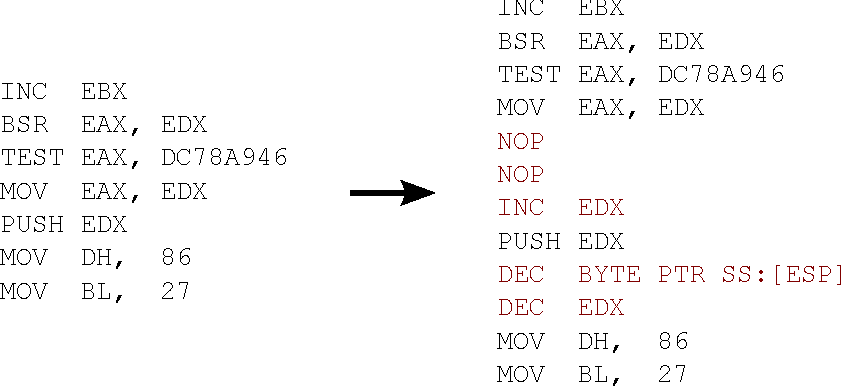
\includegraphics{obf_dci.pdf}}
    \caption{Example of dead code insertion}
    \label{fig_comp}
\end{figure}

\paragraph*{Register reassignment}
Operands of assembly code instructions are often stored in registers. The obfuscation changes the registers in which the operands of instructions are stored. The number of possible mutations this obfuscations allows can be large depending on the instructions used and number of registers available, however it can be easily circumvented via using inexact syntactic signatures.

\begin{figure}[H]
    \centering
    \scalebox{0.25}{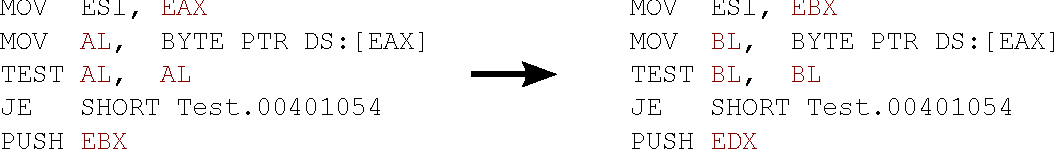
\includegraphics{obf_regswap.pdf}}
    \caption{Example of register reassignment}
    \label{fig_comp}
\end{figure}

\paragraph*{Subroutine reordering}
Or code permutation is a transformation where standalone assembly code segments such as subroutines or basic blocks can be randomly reordered to produce up to $N!$ mutations, where $N$ is the number of such segments.

\begin{figure}[H]
    \centering
    \scalebox{0.25}{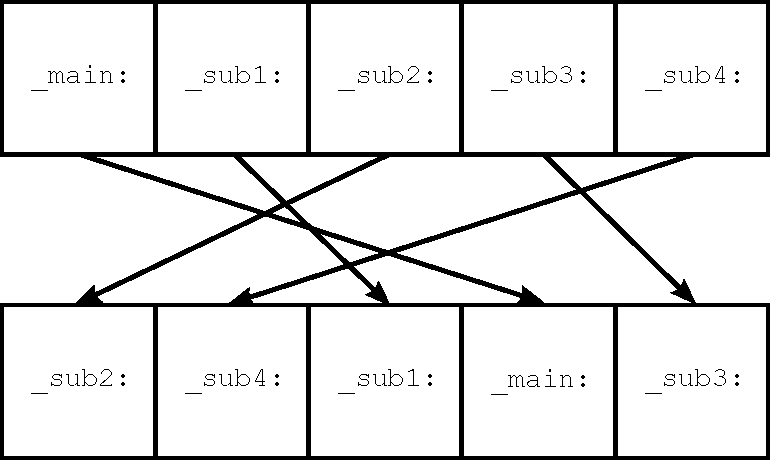
\includegraphics{obf_perm.pdf}}
    \caption{Example of subroutine reordering}
    \label{fig_comp}
\end{figure}

\paragraph*{Instruction substitution}
The effect of a single instruction in assembly code can be often emulated via a sequence of instructions. Typical examples are simple arithmetic and boolean operations which can be emulated in a number of ways each.

\begin{figure}[H]
    \centering
    \scalebox{0.25}{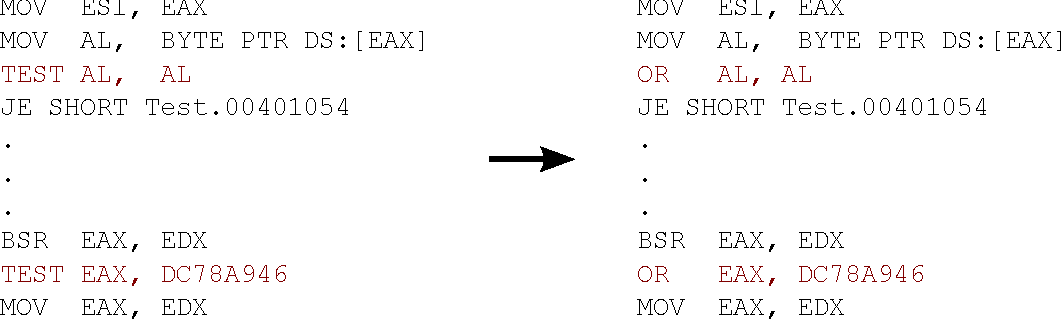
\includegraphics{obf_instrsub.pdf}}
    \caption{Example of instruction substitution}
    \label{fig_comp}
\end{figure}

\paragraph*{Code transposition}
\paragraph*{Code integration}

\subsection{Metamorphism}
\section{Syntactic Detection}
Historically malware detection techniques were centered around syntactic properties of a binary file under inspection. These methods often look for specific byte sequences in binary files and any file that contains a byte sequence that is deemed malicious is marked as malware. The advantages of this approach are speed and scalability. 
    \section{Behavioral Detection}
\chapter{Static Analysis}
\label{ch_s_analysis}
    \section{Posets and Lattices}
    \section{Abstract Interpretation}
\chapter{Formal Models}
\label{ch_models}
    \section{Tree Automata}
        \subsection{Inference}
\chapter{The LLVM Compiler Framework}
\label{ch_llvm}
    \section{Structure and Design}
    \section{Intermediate Representation}
\chapter{Detector Design and Implementation}
\label{ch_detector}
    \section{Input generation}
    \section{Taint analysis}
    \section{Classifier Inference}
    \section{Testing and Results}
\chapter{Conclusion}
\label{ch_conclusion}
    \section{Discussion}
    \section{Future Work}

%=========================================================================
 % viz. obsah.tex

  % Pouzita literatura
  % ----------------------------------------------
\ifczech
  \makeatletter
  \def\@openbib@code{\addcontentsline{toc}{chapter}{Literatura}}
  \makeatother
  \bibliographystyle{czechiso}
\else 
  \makeatletter
  \def\@openbib@code{\addcontentsline{toc}{chapter}{Literature}}
  \makeatother
  \bibliographystyle{plain}
%  \bibliographystyle{alpha}
\fi
  \begin{flushleft}
  \bibliography{literatura} % viz. literatura.bib
  \end{flushleft}

  % Prilohy
  % ---------------------------------------------
  \appendix
\ifczech
  \renewcommand{\appendixpagename}{Přílohy}
  \renewcommand{\appendixtocname}{Přílohy}
  \renewcommand{\appendixname}{Příloha}
\fi
  \appendixpage
\ifczech
  \section*{Seznam příloh}
  \addcontentsline{toc}{section}{Seznam příloh}
\else
  \section*{List of Appendices}
  \addcontentsline{toc}{section}{List of Appendices}
\fi
  \startcontents[chapters]
  \printcontents[chapters]{l}{0}{\setcounter{tocdepth}{2}}
  %\chapter{Obsah CD}
%\chapter{Manual}
%\chapter{Konfigrační soubor}
%\chapter{RelaxNG Schéma konfiguračního soboru}
%\chapter{Plakat}

 % viz. prilohy.tex
\end{document}
